\documentclass[11pt]{article}
\usepackage{amsmath}
\usepackage{tikz}
\usetikzlibrary{calc,angles,quotes,arrows.meta}
\usepackage[margin=2cm]{geometry}

% Draft reconstructions of the three Chapter 9 figures as line-only TikZ,
% for approval before replacing the OCR image crops in Chap9.tex.

\tikzset{
  edge/.style={line width=1pt},
  vlbl/.style={font=\normalsize},
  elbl/.style={font=\small},
  dotnode/.style={circle, fill=black, inner sep=2pt},
  }


\begin{document}
\begin{center}\large\textbf{Chapter 9 figures --- TikZ drafts for approval}\end{center}
\medskip

%======================================================================
% Figure 1 : the tetrahedron (diamond projection)
%======================================================================
\begin{center}
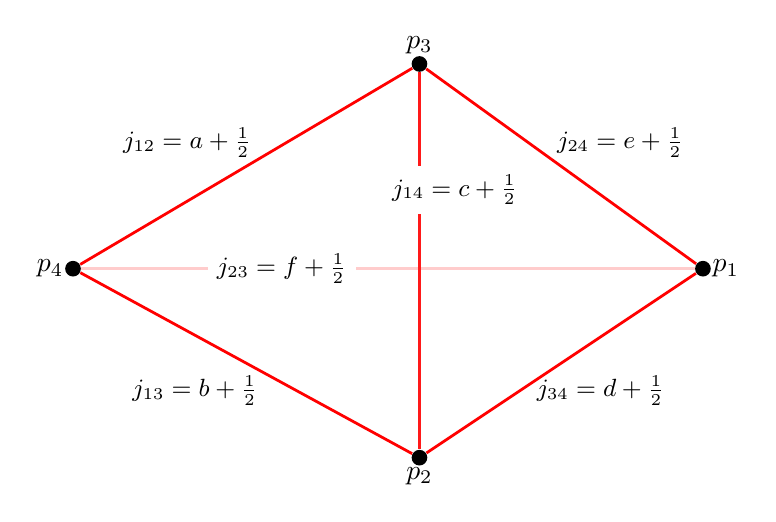
\begin{tikzpicture}[scale=1.0]
  \node[dotnode] (p3) at (0.4, 2.6) {};   % top
  \node[dotnode] (p2) at (0.4,-2.4) {};   % bottom
  \node[dotnode] (p4) at (-4, 0) {};      % left
  \node[dotnode] (p1) at ( 4, 0) {};      % right

  % six tetrahedron edges
  \draw[edge,color=red] (p4)--(p3) (p3)--(p1) (p4)--(p2) (p2)--(p1); % outer rhombus
  \draw[edge,color=red!20] (p4)--(p1);           % horizontal diagonal  j23
  \draw[edge,color=red!90] (p3)--(p2);           % vertical diagonal    j14

  % vertices
  \node[vlbl,above]      at (p3) {$p_3$};
  \node[vlbl,left]       at (p4) {$p_4$};
  \node[vlbl,right]      at (p1) {$p_1$};
  \node[vlbl,below]      at (p2) {$p_2$};

  % edge labels
  \node[elbl] at (-2.55, 1.6) {$j_{12}=a+\tfrac12$};
  \node[elbl] at ( 2.95, 1.60) {$j_{24}=e+\tfrac12$};
  \node[elbl] at (-2.45,-1.55) {$j_{13}=b+\tfrac12$};
  \node[elbl] at ( 2.7,-1.55) {$j_{34}=d+\tfrac12$};
  \node[elbl,fill=white] at (-1.35, 0) {$j_{23}=f+\tfrac12$};
  \node[elbl,fill=white] at ( 0.85, 1.00) {$j_{14}=c+\tfrac12$};
\end{tikzpicture}

\smallskip
\textit{Fig.~9.1  The tetrahedron associated with asymptotic behaviour of the $6j$ symbols.}
\end{center}

\vspace{1.2cm}

%======================================================================
% Figure 2 : Edmonds' angle theta
%======================================================================
\begin{center}
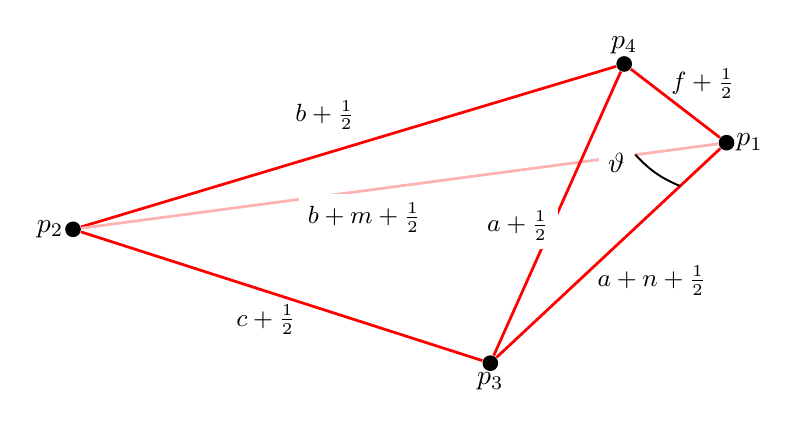
\begin{tikzpicture}[scale=1.0]
  \node[dotnode] (p2) at (-4.6,-0.2) {};
  \node[dotnode] (p4) at ( 2.4, 1.9) {};
  \node[dotnode] (p1) at ( 3.7, 0.9) {};
  \node[dotnode] (p3) at ( 0.7,-1.9) {};

  % six edges
  \draw[edge,color=red] (p2)--(p4);           % b+1/2
  \draw[edge,color=red] (p4)--(p1);           % f+1/2
  \draw[edge,color=red] (p2)--(p3);           % c+1/2
  \draw[edge,color=red!30] (p2)--(p1);           % b+m+1/2
  \draw[edge,color=red] (p3)--(p1);           % a+n+1/2
  \draw[edge,color=red] (p3)--(p4);           % a+1/2

  % angle theta at p1 between edges p1-p3 (a+n+1/2) and p1-p2 (b+m+1/2)
  \path (p1) -- (p3) coordinate[pos=0.18] (t3);
  \path (p1) -- (p2) coordinate[pos=0.13] (t2);
  \draw[line width=0.7pt] (t3) to[bend left=12] (t2);
  \node[vlbl,fill=white] at ($(p1)+(-1.4,-0.25)$) {$\vartheta$};

  % vertices
  \node[vlbl,left]  at (p2) {$p_2$};
  \node[vlbl,above] at (p4) {$p_4$};
  \node[vlbl,right] at (p1) {$p_1$};
  \node[vlbl,below] at (p3) {$p_3$};

  % edge labels
  \node[elbl] at (-1.4, 1.25) {$b+\tfrac12$};
  \node[elbl] at ( 3.4,1.65) {$f+\tfrac12$};
  \node[elbl] at (-2.15,-1.35){$c+\tfrac12$};
  \node[elbl,fill=white] at (-0.9,-0.05) {$b+m+\tfrac12$};
  \node[elbl,fill=white] at ( 1.05,-0.15) {$a+\tfrac12$};
  \node[elbl] at ( 2.75,-0.85) {$a+n+\tfrac12$};
\end{tikzpicture}

\smallskip
\textit{Fig.~9.2  The angle $\vartheta$ which enters Eq.~9.9(14).}
\end{center}

\vspace{1.2cm}

%======================================================================
% Figure 3 : spherical-triangle angle construction at p1
%======================================================================
\begin{center}
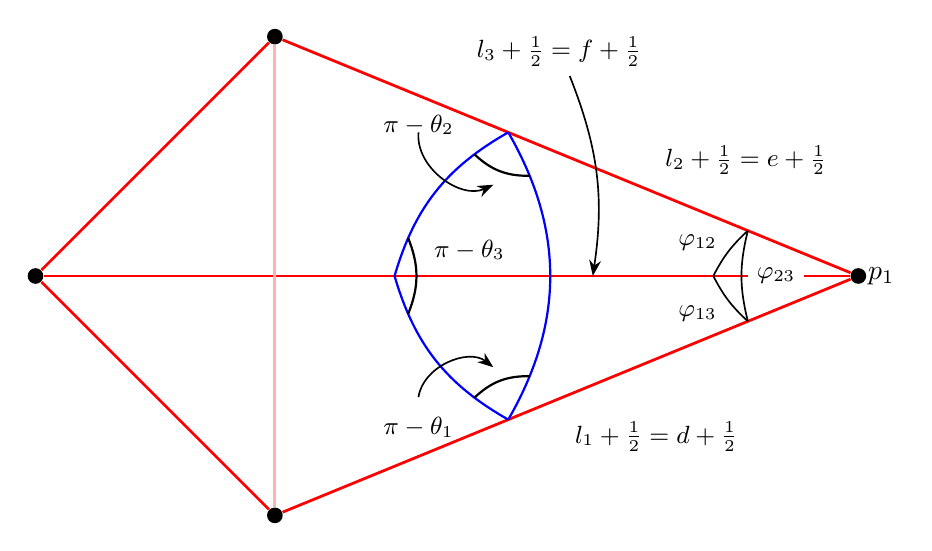
\begin{tikzpicture}[scale=0.95]
  \node[dotnode]  (Al) at (-5, 0) {};      % far left vertex
  \node[dotnode]  (At) at (-1.8, 3.2) {};  % top vertex
  \node[dotnode]  (Ab) at (-1.8,-3.2) {};  % bottom vertex
  \node[dotnode]  (p1) at ( 6, 0) {};      % right apex

  % outer kite / tetrahedron seen edge-on
  \draw[edge,color=red] (Al)--(At)--(p1)--(Ab)--(Al);
  \draw[edge,color=red] (Al)--(p1);           % horizontal axis (edge p1--Al)
  \draw[edge,color=red!30] (At)--(Ab);           % horizontal axis (edge p1--Al)

  % points where the small sphere around p1 meets the three edges to At,Ab,Al
  \coordinate (Vu) at ($(p1)!0.60!(At)$);
  \coordinate (Vl) at ($(p1)!0.60!(Ab)$);
  \coordinate (Vm) at (-0.2,0);      % on the axis, left vertex of spherical triangle

  % straight meridians p1 -> vertices (already partly along kite edges/axis)
  % spherical-triangle edges (arcs)
  \draw[line width=0.8pt,color=blue] (Vu) to[bend right=22] node[pos=0.2] (au1) {}node[pos=0.8] (am1) {}  (Vm);   % upper-left edge
  \draw[line width=0.8pt,color=blue] (Vm) to[bend right=22]  node[pos=0.2] (am2) {}  node[pos=0.8] (al1) {} (Vl);   % lower-left edge
  \draw[line width=0.8pt,color=blue] (Vu) to[bend left=30] node[pos=0.15] (au2) {} node[pos=0.85] (al2) {}  (Vl);   % right edge (bulges toward p1)
\draw[line width=0.8pt] (au1.center) to[bend right=22] (au2.center);
\draw[line width=0.8pt] (al1.center) to[bend left=22] (al2.center);
\draw[line width=0.8pt] (am1.center) to[bend left=22] (am2.center);

  % small angle arcs at p1 (phi_ik between the three meridians)
  \path (p1) -- (Vu) coordinate[pos=0.3] (u1);
  \path (p1) -- (Vl) coordinate[pos=0.3] (l1);
  \path (p1) -- (Vm) coordinate[pos=0.30] (m1);
  \path (p1) -- (Vu) coordinate[pos=0.40] (u2);
  \path (p1) -- (Vl) coordinate[pos=0.40] (l2);
  \draw[line width=0.6pt] (u1) to[bend right=10] (m1);   % phi_12
  \draw[line width=0.6pt] (m1) to[bend right=10] (l1);   % phi_13
  \draw[line width=0.6pt] (u1) to[bend right=14]  (l1);   % phi_23 (wider)

  % phi labels near p1
  \node[elbl] at (3.85, 0.45) {$\varphi_{12}$};
  \node[elbl] at (3.85,-0.50) {$\varphi_{13}$};
  \node[elbl,fill=white] at (4.9, 0) {$\varphi_{23}$};

  % spherical-triangle vertex (dihedral) angles pi - theta_i
  \draw[-{Stealth[length=2mm]},line width=0.6pt]  ($(Vu)+(-1.2,0)$) to[bend right=60]  ($(Vu)+(-0.2,-0.7)$);
  \node[elbl] at ($(Vu)+(-1.2,0.1)$) {$\pi-\theta_2$};
  \node[elbl] at ($(Vm)+(1.0,0.35)$) {$\pi-\theta_3$};
   \draw[-{Stealth[length=2mm]},line width=0.6pt]  ($(Vl)+(-1.2,0.3)$) to[bend left=60]  ($(Vl)+(-0.2,0.7)$);
  \node[elbl] at ($(Vl)+(-1.2,-0.1)$) {$\pi-\theta_1$};

  % edge (l_i) labels with pointer arrows
  \node[elbl] (Lf) at (2, 3) {$l_3+\tfrac12=f+\tfrac12$};
  \draw[-{Stealth[length=2mm]},line width=0.6pt] (Lf) to[bend left=15] (2.45,0);
  \node[elbl] at (4.5, 1.55) {$l_2+\tfrac12=e+\tfrac12$};
  \node[elbl] at (3.3,-2.15) {$l_1+\tfrac12=d+\tfrac12$};

  \node[vlbl,right] at (p1) {$p_1$};
\end{tikzpicture}

\smallskip
\textit{Fig.~9.3  Geometrical interpretation of the angles in Eqs.~9.9(20)--9.9(23).}
\end{center}

\end{document}
